\section{LHCb Experiment}

The LHCb experiment is one of the 7 experiments located on the Large Hadron Collider. It was built in order to search for indirect evidence of new physics phenomona through the study of CP violation and rare decays for hadrons that contain b and c quarks.

In proton collisions provided by the LHC heavy quark pairs are predominantly produced at small angles to the beam pipe. The dominant production mechanisms that produced bbbar pairs are quark anti-quark annihilation, gluon-gluon fusions and  gluon splitting as shown in the Feynman diagrams in Figure X. There must be some other reason why these processes lead to the quarks being boosted along the beam pipe and I shall explain that here. Once the bbbar pairs are produced the quarks hadronise(?), in to Bs, Bd, B+ and many others and the decays of these hadrons have some specific characteristics. B-mesons tend to have long lifetime around 1 ps therefore travel ~1cm from the interaction vertex where they were produced before decaying at a secondary vertex. Since b quarks are heavy quarks, the hadrons they for can decay into a large range of different particles from light particle such as electrons and photons to heavier particles like kaons, muons and D mesons. The experiment was designed around the production characteristics of bbbar pairs and to enable precise measurements of b hadron decays. 

The LHCb experiment was built as a single arm forward spectrometer, with an angular coverage of 10 to 300 mrad in the vertical direction and 10 to 250 mrad in the horizontal direction relative the the beam pipe. This angular coverage what chosen to exploit the small angles relative the the beam pipe that bbbar pairs are produced at. A cross-section of the detector is shown in Figure \ref{fig:LHCb_detector}, where a right handed coordinate system is used. Protons collide at the interaction point on the left hand side of the diagram, the products of the collisions then travel through the detector leaving information in the different sub detectors along the length of the detector. The information deposited in the sub detectors are reconstructed to determine what happened in the proton collisions. The sub detectors can be classified in to two main categories; tracking system and particles identification system .

The tracking system is make up to the vertex locator (VELO), the magnet, the TT and the tracking stations T1-3. The VELO is designed to provide precise tracking measurements to identity the primary and secondary vertices characteristic of b-hadron decays in order to determine accurate lifetimes of b-hadrons. The magnet and tracking stations are combined to give high momentum resolution which is necessary to achieve good mass resolution which is used to distinguish between different b hadrons and separate signal and background decays.

The particle identification detectors provide complementary information about the identity of particles passing through them which enables the many different decay products of b-hadrons to be identified and the hadron to be accurately reconstructed. The RICH detectors provide information about these types of particles, the two calorimeters give informations that separates electrons, positrons and photons and from hadrons. Finally the muons stations at the furthest point from the integration point identify muons as the name suggests. 

The measurement of of decays of heavy hadrons requires accurate reconstruction of secondary vertices, this is achieved in part by the tracking systems however another aspect of the LHCb experiment deigns that enables this is the luminosity the experiment operates at. The LHC was designed to deliver a luminosity of X, proton collisions at this luminosity leads to a large amount of pile up. Pile up is stuff from the decay that is not interesting and is close to the beam pipe, therefore in the LHCb acceptance and makes it hard to accurately reconstruct secondary verticies. Therefore LHCb operates at a lower luminosity of ~ X in order to reduce the amount of pile up and enable accurate reconstruction of b hadron decays. 





\begin{figure}[tb] 
  \centering    
  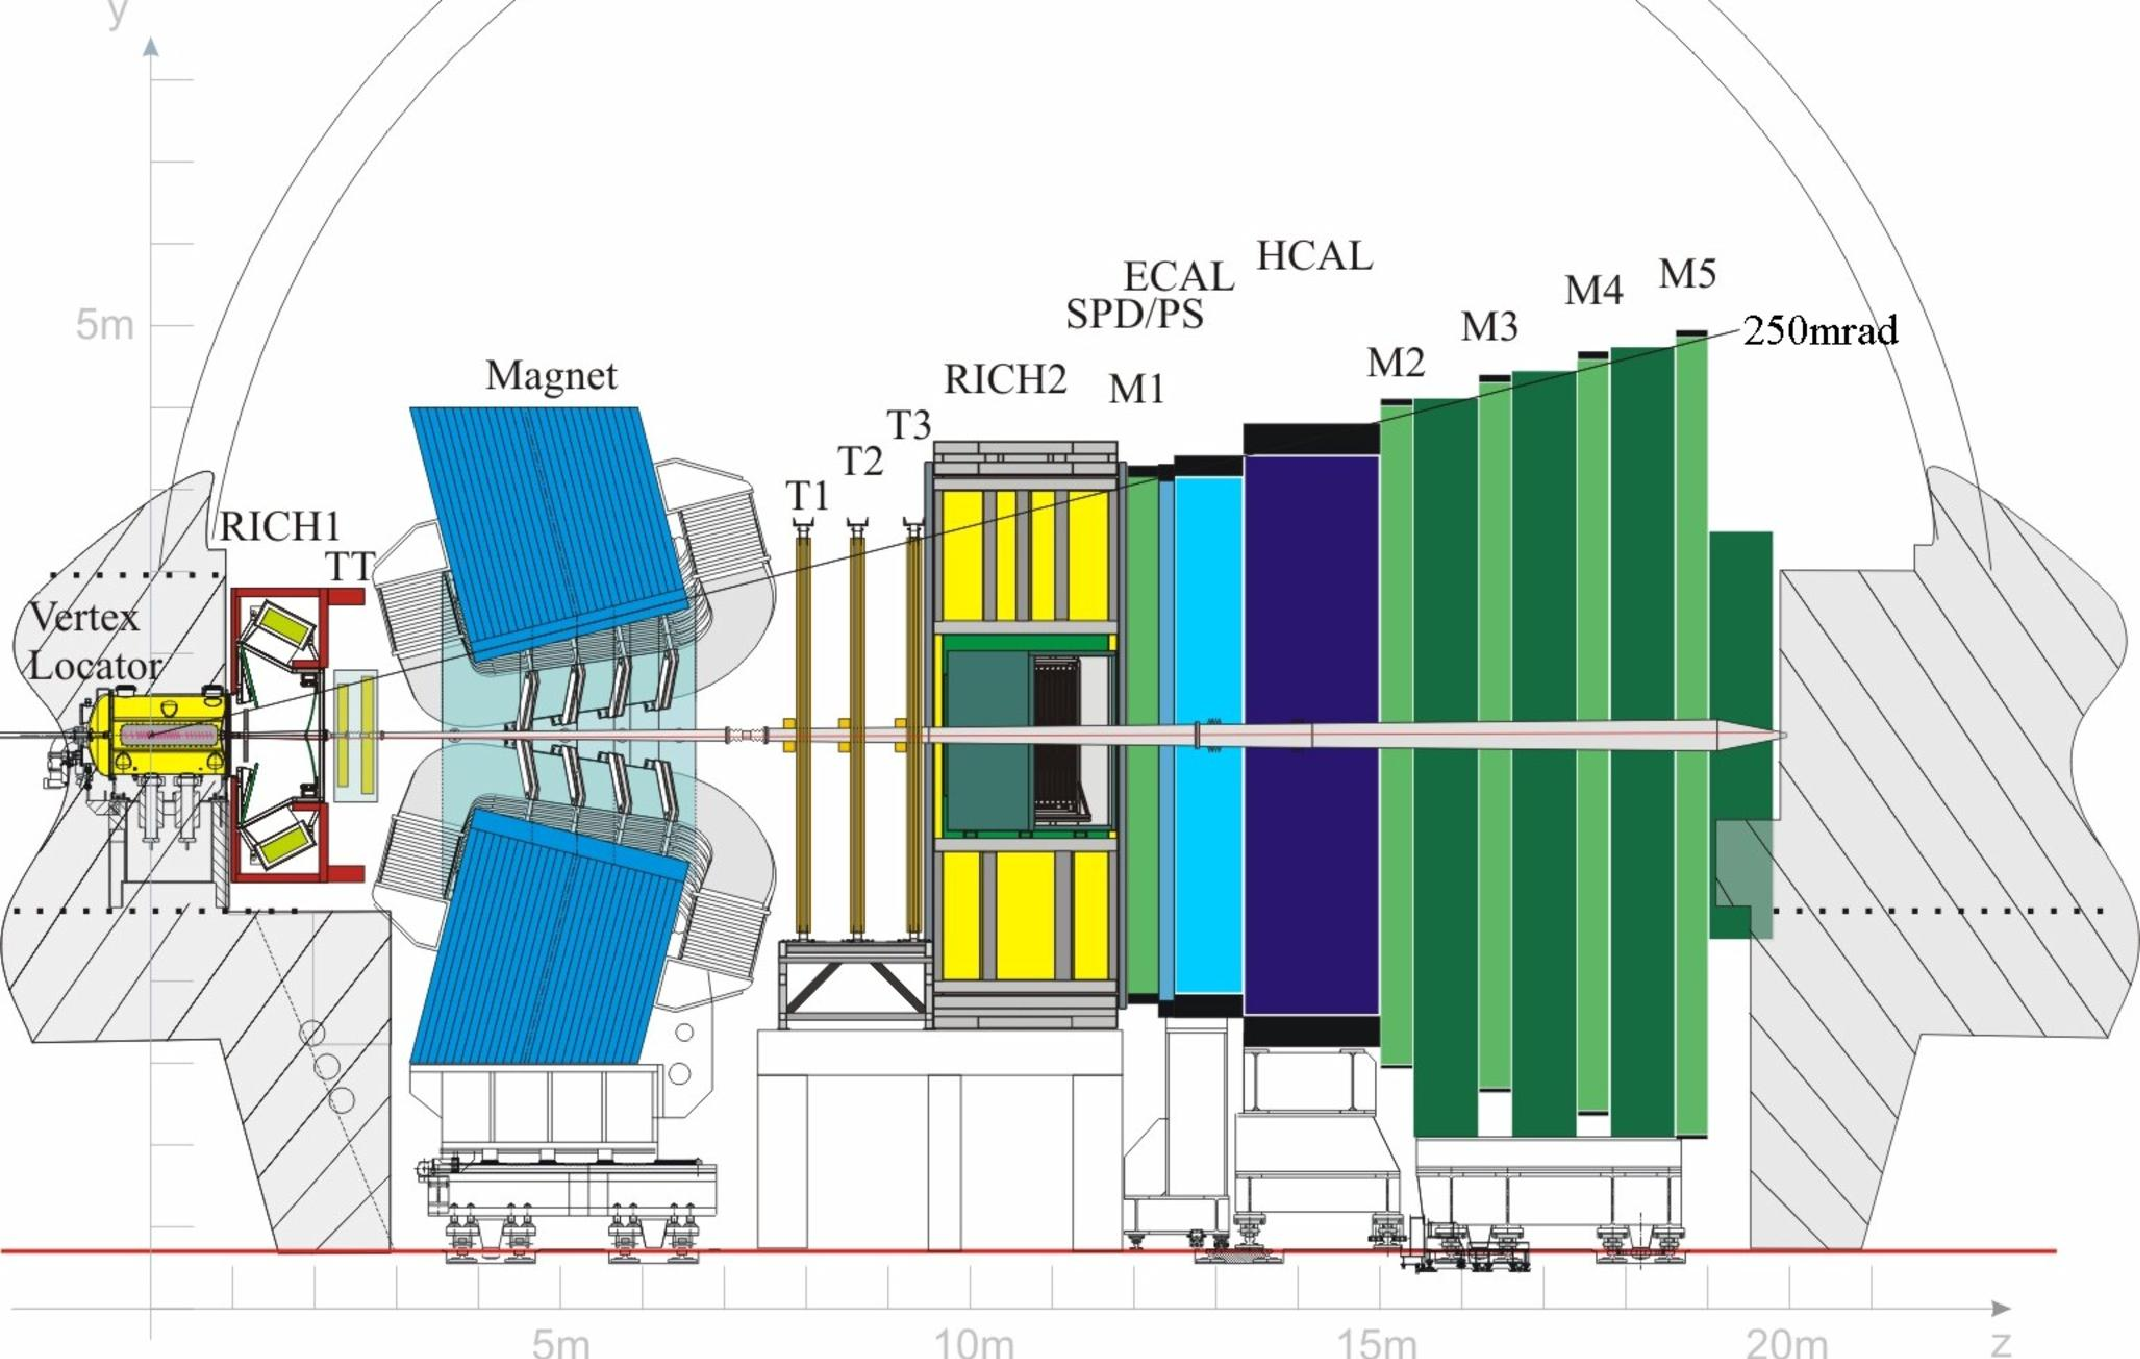
\includegraphics[ width=1.0\textwidth]{LHCb_layout.png}
  \caption{Cross section of the LHCb detector \cite{LHCb:2003ab}.}
  \label{fig:LHCb_detector}
\end{figure}




\begin{figure}[tb] 
  \centering    
  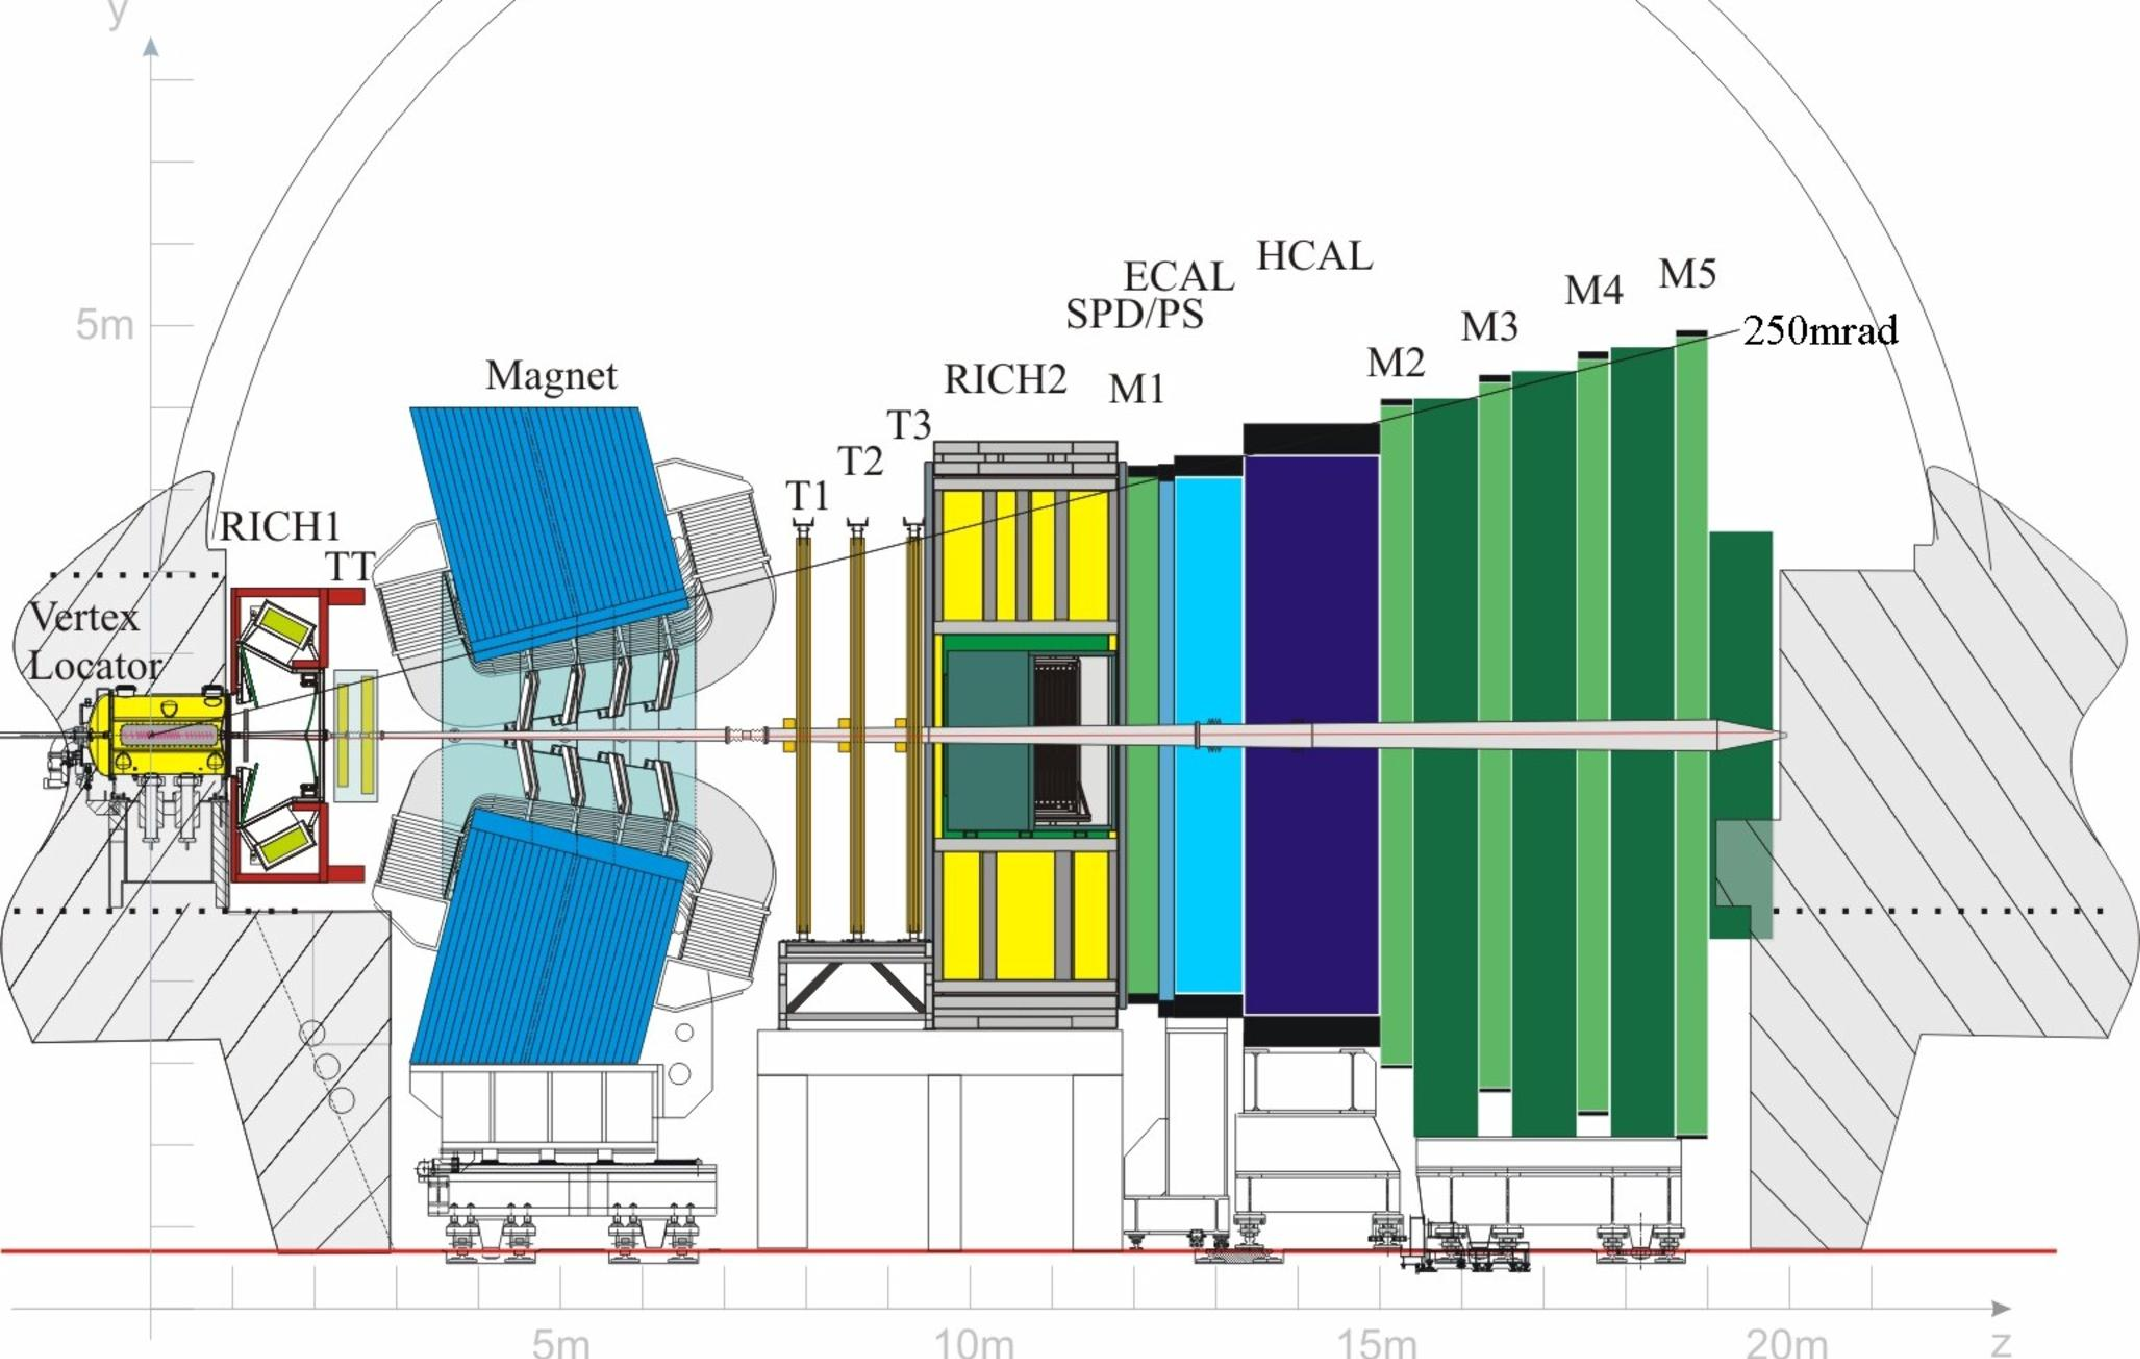
\includegraphics[ width=1.0\textwidth]{LHCb_layout.png}
  \caption{Simulated angular distribution for b-quark production at the LHC, angles are relative the the beam pipe with $\theta =0$ in the forward direction and$\theta = \pi$  in the backward direction \cite{Amato:1998xt}.}
  \label{fig:LHCb_detector}
\end{figure}


\subsection{Tracking}


\subsubsection{VELO}



\begin{figure}[tb] 
  \centering    
  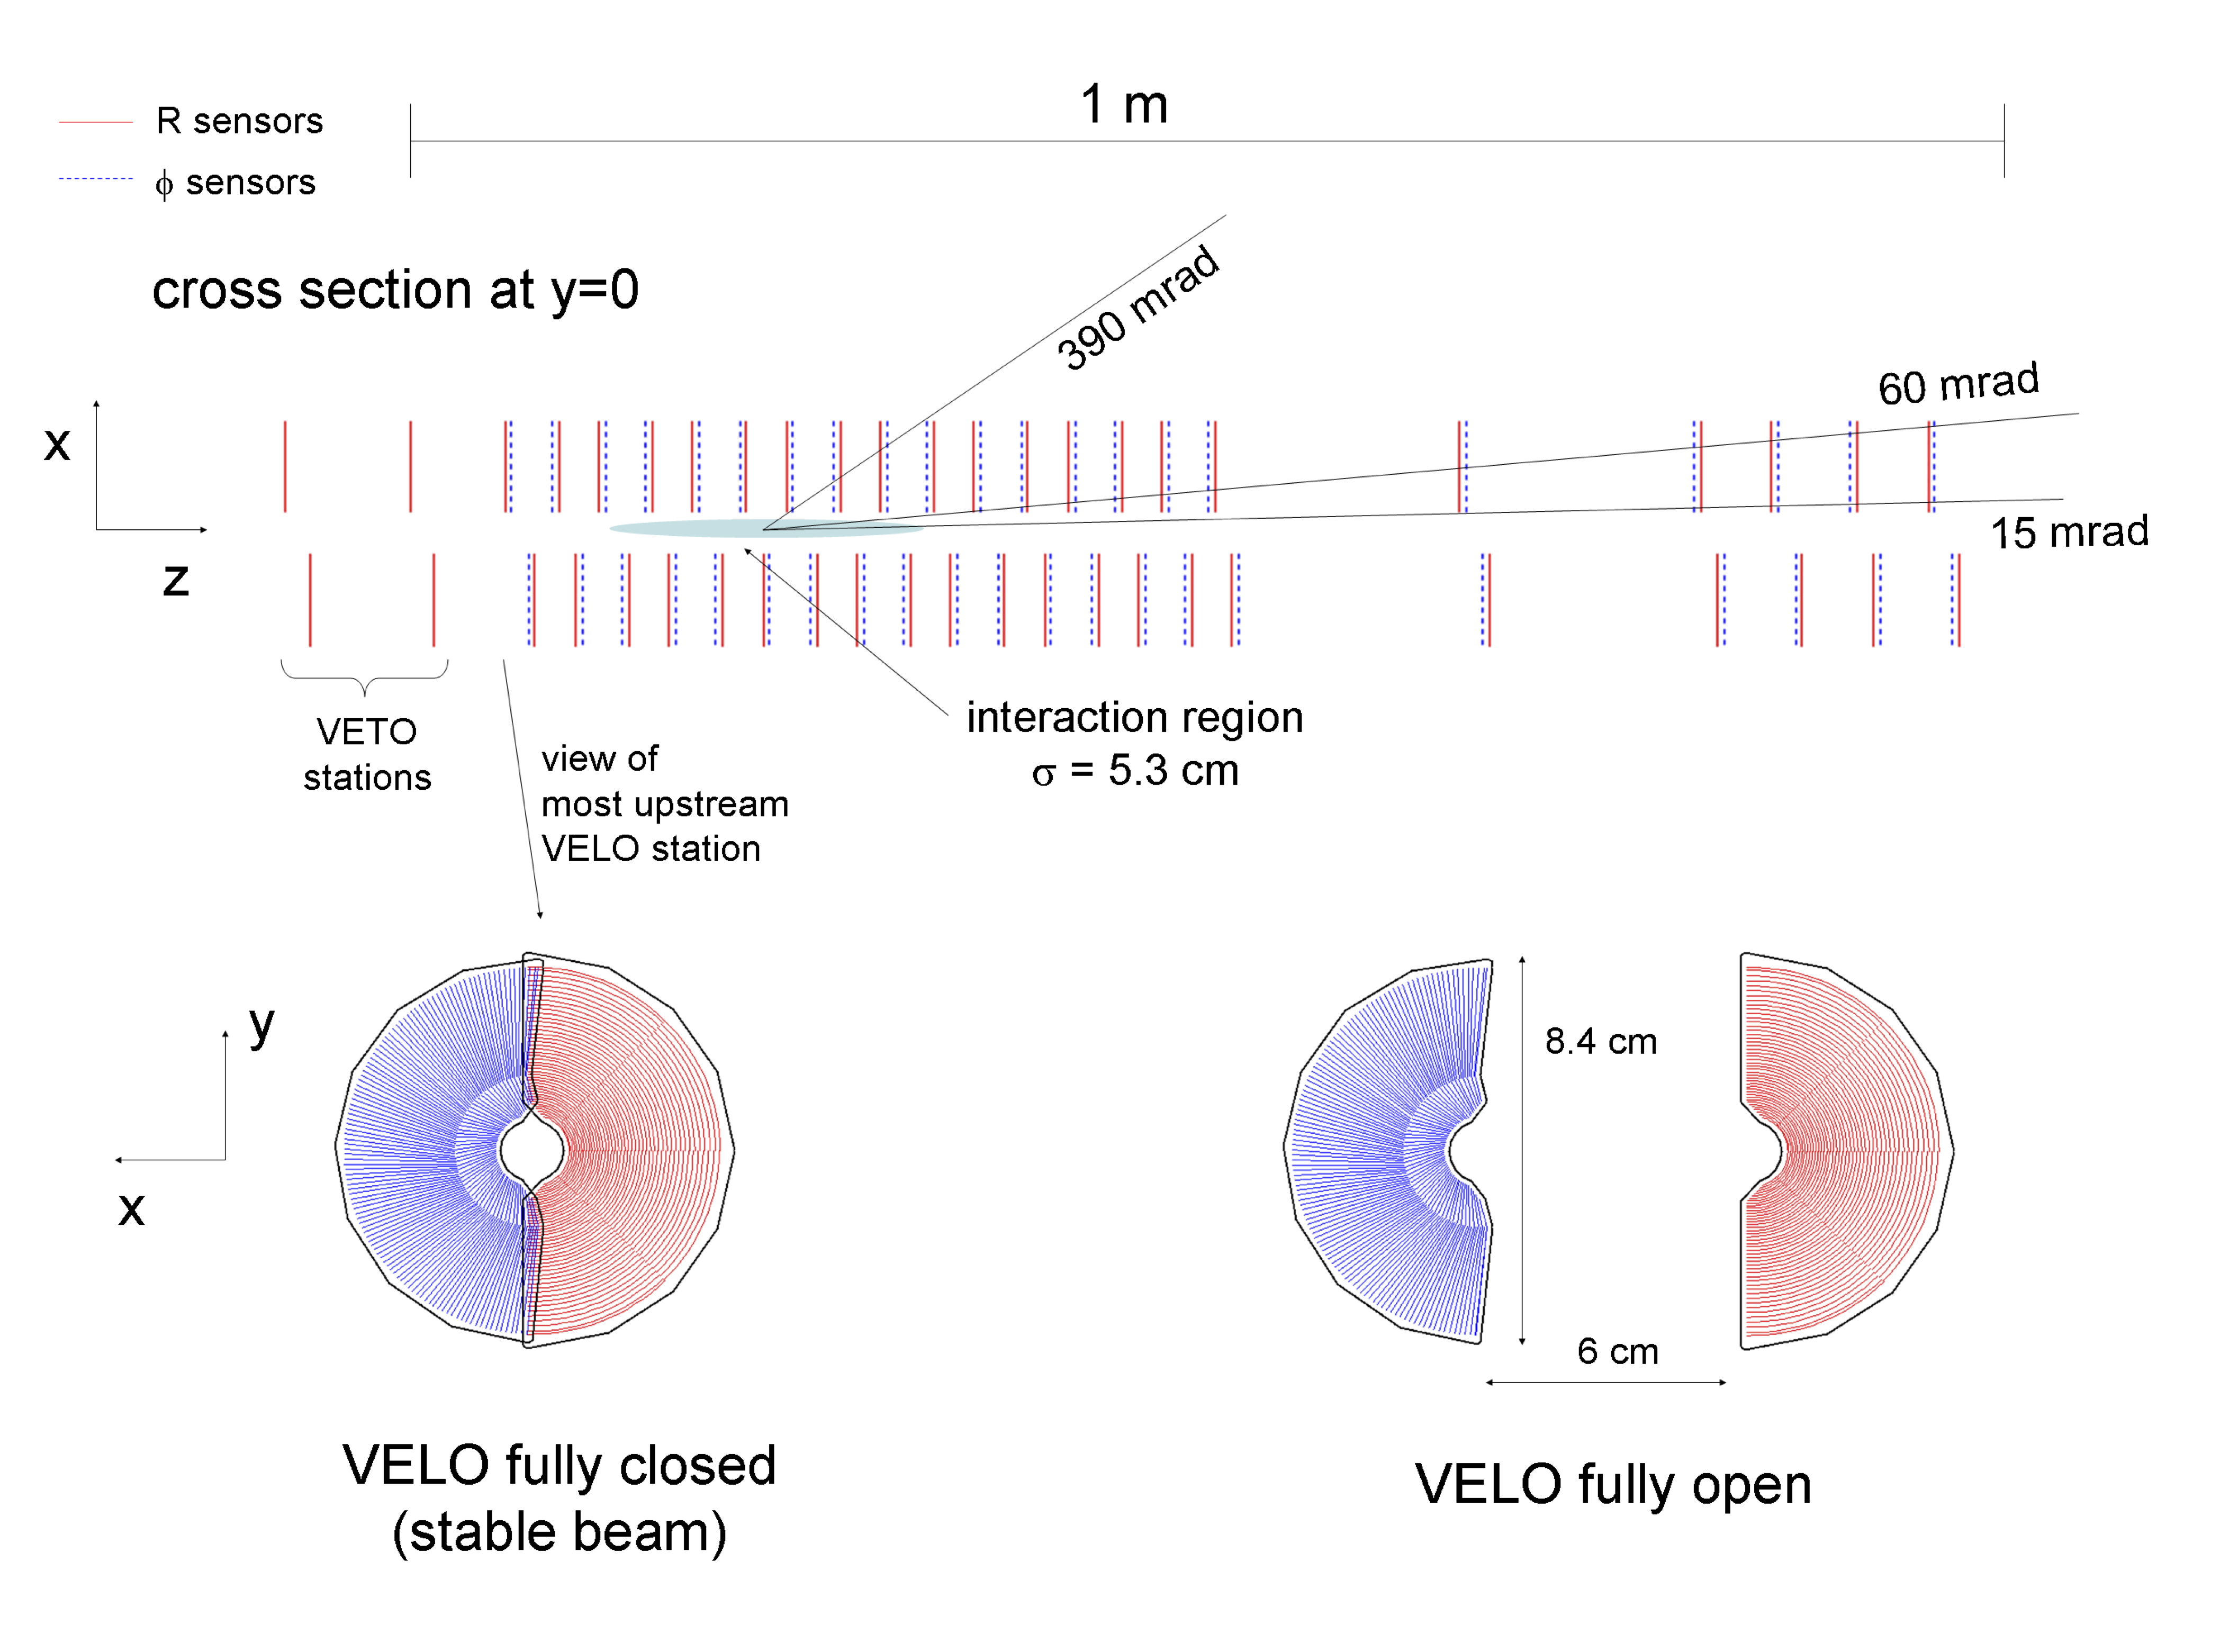
\includegraphics[ width=1.0\textwidth]{velo.png}
  \caption{The velo \cite{Alves:2008zz}.}
  \label{fig:velo}
\end{figure}

\begin{figure}[tb] 
  \centering    
  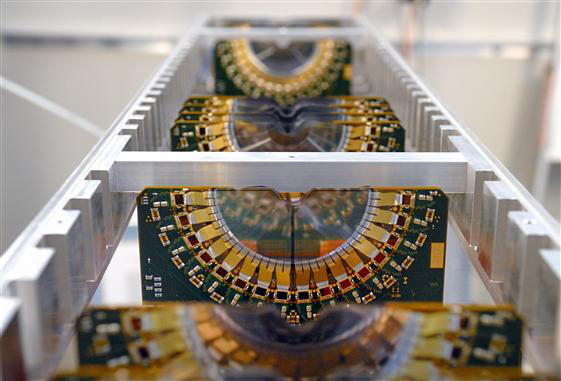
\includegraphics[ width=1.0\textwidth]{Velo_photo.jpg}
  \caption{The velo Soure: LHCb.}
  \label{fig:velo_photo}
\end{figure}

\begin{figure}[tb] 
  \centering    
  
\includegraphics[ width=1.0\textwidth]{placeholder.jpeg}
  \caption{The velo sensor \cite{Alves:2008zz}.}
  \label{fig:velo_sensor}
\end{figure}

\subsubsection{Magnet}

\subsubsection{Tracking Stations} %Or split us the TT and T1-3.

\subsubsection{Track resconstruction and preformance}


\subsection{Particle Identification}
\subsubsection{RICH}
\subsubsection{Calrimeters}
\subsubsection{Muon Stations}
\subsubsection{Combined PID information and performance}

\subsection{Trigger and event filtering}

\subsection{MC and Software}

\subsection{LHCb data collected so far}

\begin{figure}[tb] 
  \centering    
  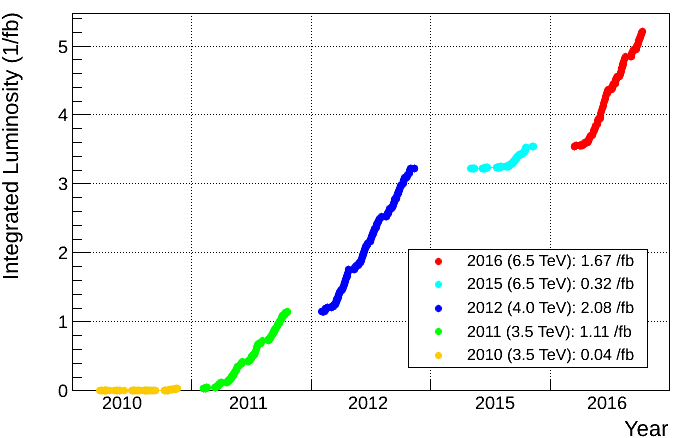
\includegraphics[ width=1.0\textwidth]{IntegratedLumiCumul.png}
  \caption{Source: LHCb.}
  \label{fig:cumulative_lumi}
\end{figure}

\begin{figure}[tb] 
  \centering    
  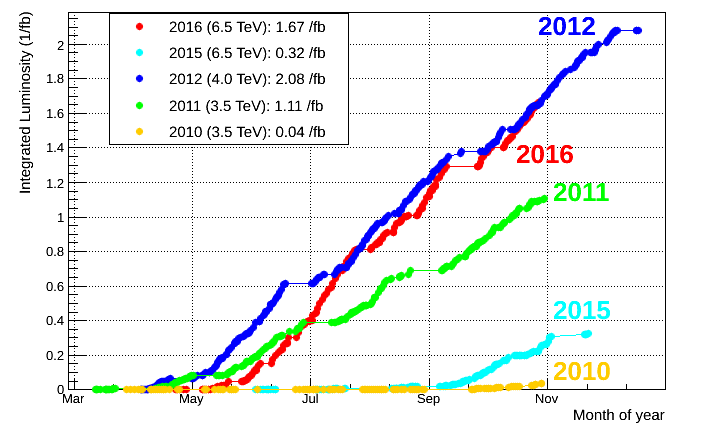
\includegraphics[ width=1.0\textwidth]{IntLumiRun1-2.png}
  \caption{Source: LHCb.}
  \label{fig:yearly_lumi}
\end{figure}
